\chapter{Doxorubicin-induced stress in cardiomyocytes results in RNA localization changes}\label{chap:chapter2}

\section{Introduction}

Doxorubicin (DOX) was once one of the most effective broad-spectrum anti-cancer anthracycline antibiotics\cite{kalyanaramanTeachingBasicsMechanism2020,youngAnthracyclineAntineoplasticDrugs1981} with particular efficacy against solid malignancies such as lung and breast cancer, as well as hematologic neoplasia\cite{sheibaniDoxorubicinInducedCardiotoxicityOverview2022,yuRecentProgressDoxorubicininduced2018}. However, DOX's propensity to cause cardiac damage in patients has led to significant limitations in its clinical use\cite{rahmanAnthracyclineinducedCardiotoxicityCardiacsparing2007}. There are two known mechanisms of action by which DOX acts in cells\cite{teweyAdriamycininducedDNADamage1984}: generation of reactive oxygen species via potential interactions with oxidation reaction pathways which then damage lipid membranes, disrupt mitochondrial function, induce DNA damage and triggers apoptotic pathways; and direct interaction with DNA topoisomerase II to induce single-stranded and double-stranded breaks. The exact mechanism by which DOX induces heart failure is unclear, but significant evidence suggests cardiomyocyte injury driven by oxidative stress as a major factor\cite{asensio-lopezDoxorubicininducedOxidativeStress2017,sheibaniDoxorubicinInducedCardiotoxicityOverview2022,simunekAnthracyclineinducedCardiotoxicityOverview2009,xiongProtectiveEffectBerberine2018,xuEffectsDoxorubicinMyocardium2001}. Specifically, DOX causes stress and dysfunction in multiple cellular compartments in cardiomyocytes such as mitochondria, Sarco/endoplasmic reticulum (SER), deficiencies in calcium signaling, and lipid degradation at the cellular membrane\cite{rawatDoxorubicininducedCardiotoxicityUpdate2021}. There is growing evidence that DOX not only interacts with DNA, but also with some affinity to double-stranded RNAs\cite{rubioDoxorubicinBindsDuplex2016}, rRNAs\cite{marcheschiSelectionCharacterizationSmall2009} and RNA aptamers\cite{bagalkotAptamerDoxorubicinPhysical2006}.

Having established Bento's utility to characterize RNA localization in cell lines (see Chapter \ref{chap:chapter 1}), we applied Bento to doxorubicin-treated and untreated cardiomyocytes, a cell line model for these cardiomyopathies. We performed single molecule spatial transcriptomics (Molecular Cartography) on doxorubicin-treated and untreated cardiomyocytes to measure consequential differences across multiple classes of phenotypes in a single experiment: RNA localization, gene expression, cell morphology.

\section{Results}

We designed a panel of 100 genes to profile with spatial transcriptomics, capturing pathways for cardiomyocyte health and function\cite{mahBentoToolkitSubcellular2022}. These include genes involved in cardiomyocyte contraction and conduction; cellular cytoskeletal pathways including myofibril assembly and cytoskeleton components; and also mitochondrial function to capture perturbations to oxidative metabolism. We reasoned that we could recapitulate known dysfunction of subcellular domains in cardiomyocytes upon DOX stress and measure novel RNA localization phenotypes that are not explained by expression changes alone.

\begin{figure}[p]
    \centering
    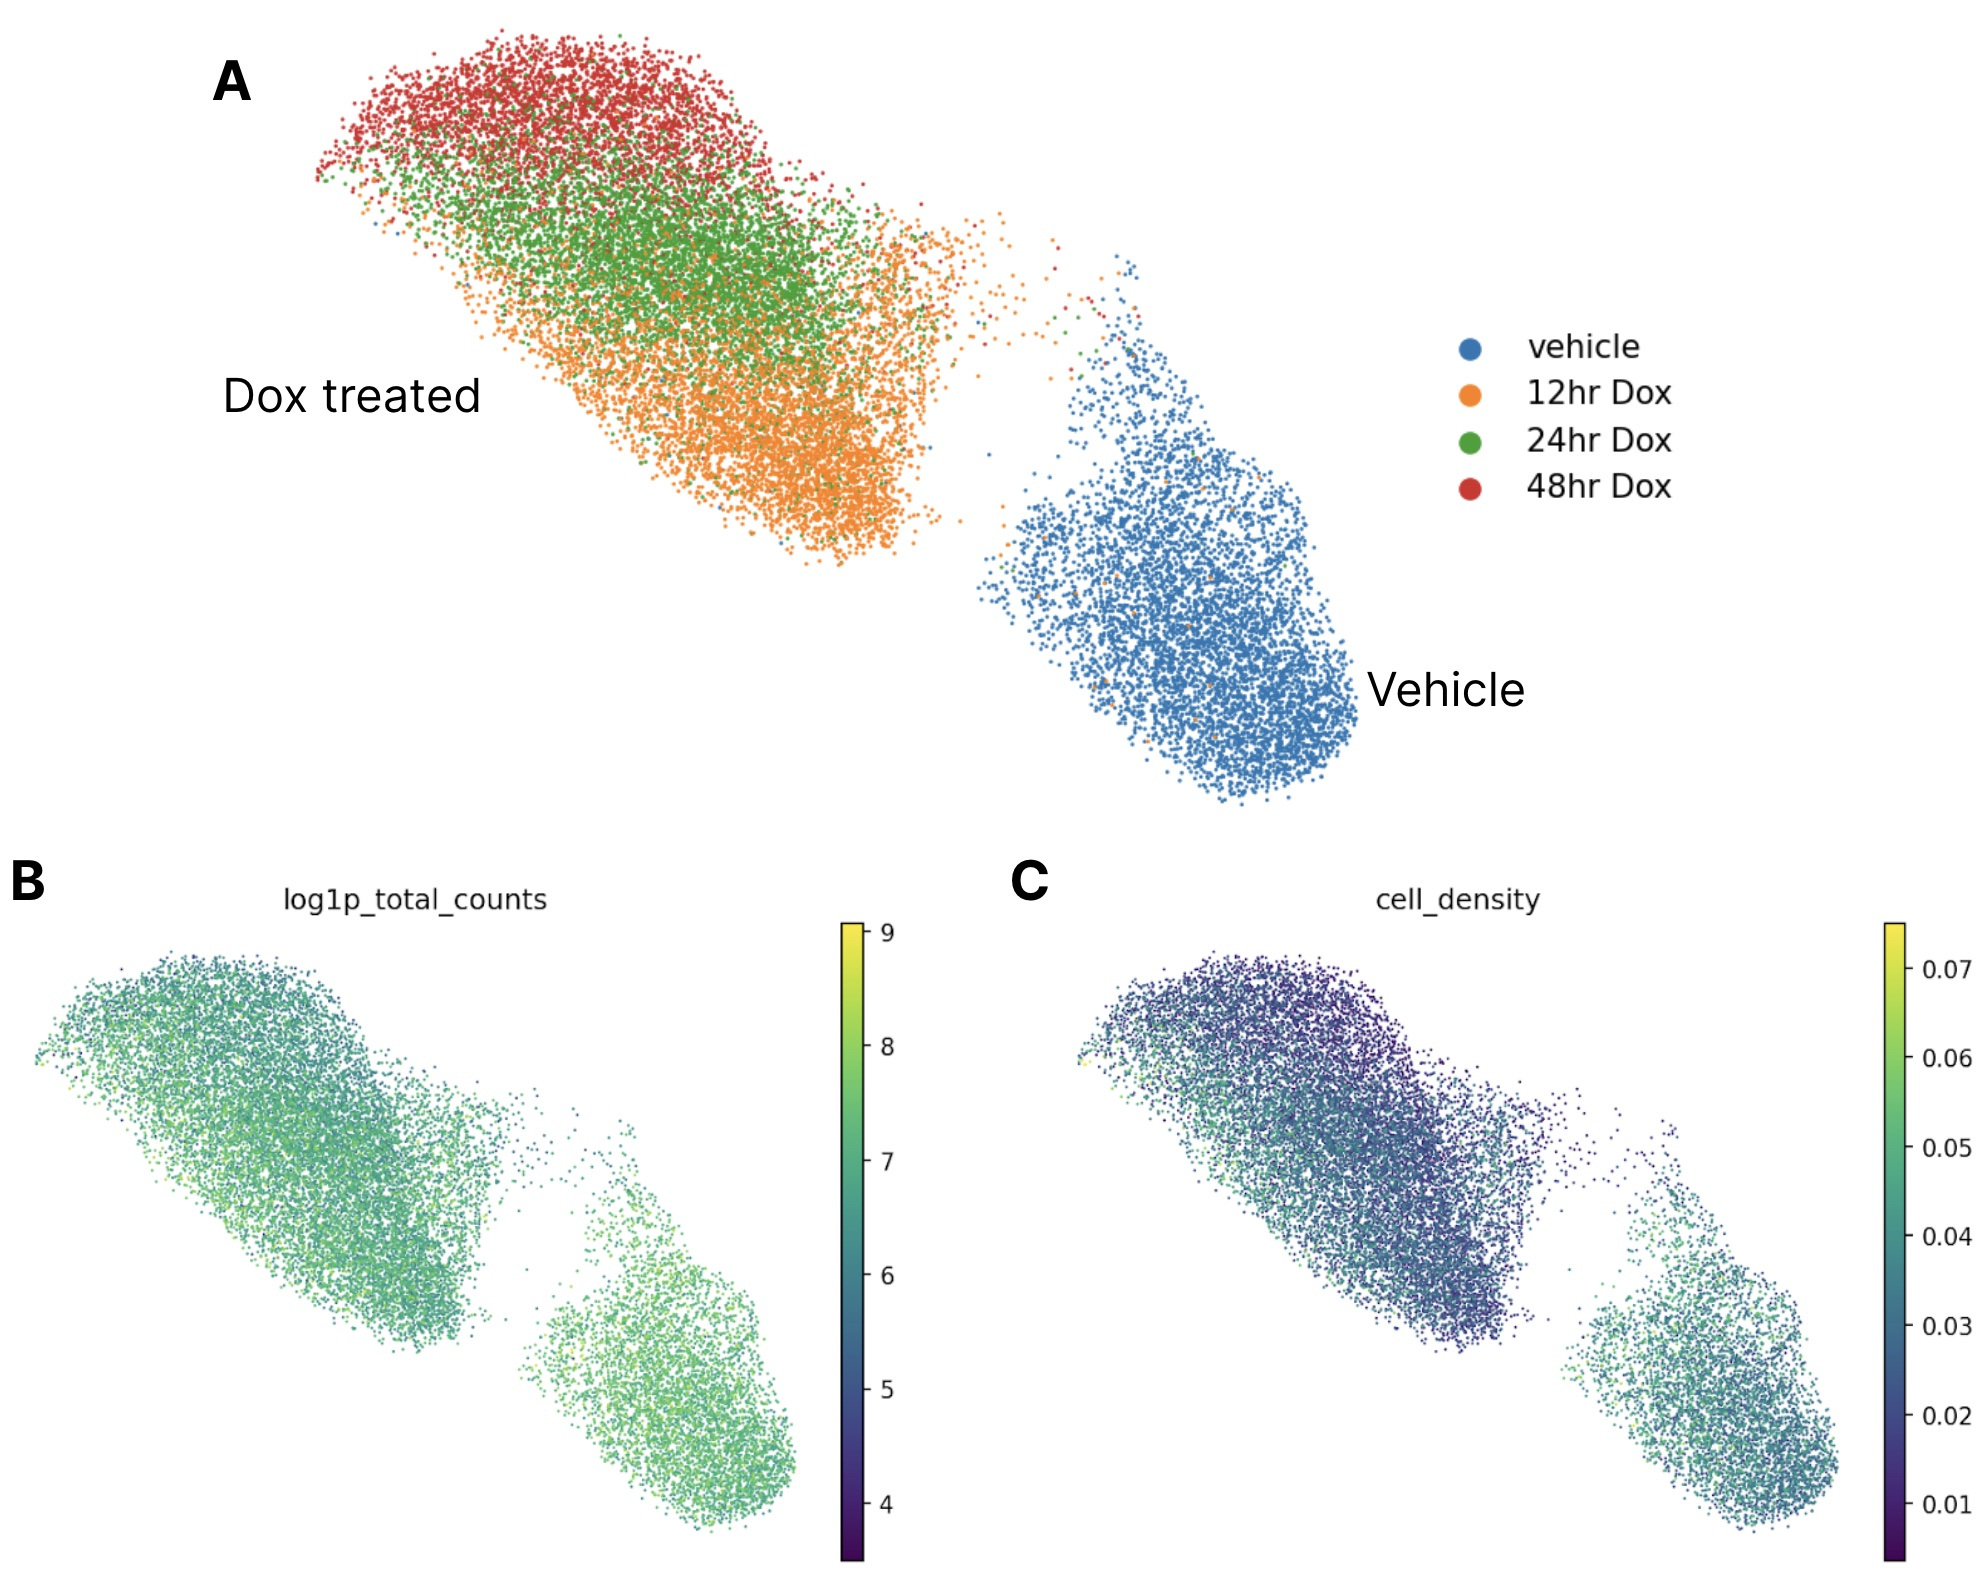
\includegraphics[width=\textwidth]{2_figures-and-files/Fig1.jpg}
    \caption[Single-cell expression of doxorubicin-treated caradiomyocytes time points]{\textbf{Single-cell expression of doxorubicin-treated caradiomyocytes time points} A. UMAP projection of single-cell expression of vehicle and doxorubicin-treated cardiomyocytes across vehicle, 12 hour, 24 hour, and 48 hour time points. Two replicates per time point. B. UMAP projection of single-cells colored by log-scaled total RNA expression and C. transcript density (transcript count divided by cell area).}
    \label{fig:Doxorubicin treatment single-cell expression}
\end{figure}

We utilized a chemically-defined protocol to differentiate human induced pluripotent stem cells (iPSCs) into beating cardiomyocytes and treated them with either DMSO (vehicle) or 2.5 uM DOX for twelve hours, 24 hours, or 48 hours before fixation (Methods). Each treatment had 2 replicates. Single molecule spatial transcriptomes were measured by Resolve Bioscience using Molecular Cartography. The resulting data was segmented using ClusterMap\cite{heClusterMapMultiscaleClustering2021} for cell boundaries and Cellpose\cite{stringerCellposeGeneralistAlgorithm2021} for nuclei boundaries. Non-myocytes were filtered out using SLC8A1 as a canonical marker for cardiomyocytes (Methods, Supp. Fig. 1A). 


Comparing vehicle and DOX treated cardiomyocytes, we found vehicles cells to cluster distinctly from all DOX treated cells (Fig. 1) and DOX treated cells forming a duration-dependent expression gradient from 12-48 hours. Notably, transcript density i.e. transcript count dividedby cell area, decreases with treatment duration. Differential expression analysis of each timepoint relative to vehicle indicate that DOX induces cellular stress as expected. NPPA and NPPB are important biomarkers in clinical cardiology that become upregulated during cardiac stress\cite{manStructureFunctionNppa2018,songAtrialNatriureticPeptide2015}. Elevated levels of NPPB have been used to diagnose patients with doxorubicin induced cardiotoxicity and elevated levels of NPPB also correlate with severity of heart failure. An increase in NPPA and NPPB levels upon Doxorubicin exposure at 24 and 48 hours indicates that the cardiomyocytes have transitioned to a state of cellular stress (Fig. 2A,B).

We then restricted our analysis to focus on the 12 hour treatment and vehicle for spatial analyses via Bento. Poor segmentation quality for the other timepoints limited the precision and accuracy of 2-dimensional spatial analysis algorithms. We identified subcellular domains in vehicle and 12 hour DOX treated cardiomyocytes using RNAflux, clustering the domains into four fluxmap domains (Fig. 2C). Enrichment of location-specific gene expression aligned domains to the nucleus (nuclear pore, nucleolus, and nucleus), ERM and OMM, ER lumen, and cytosol respectively (Fig. 2C \& D, Supp. Fig. 1C). Comparing the gene composition in each domain, we observe an overall localization bias towards both the nucleus and ERM/OMM in vehicle treated cells (**Fig. 2E top**), in agreement to prior poly(A) smFISH studies\cite{lewisLocalizationTranscriptsTranslation2018}. However, RNA in the DOX treated cardiomyocytes demonstrated a shift in average RNA localization away from the ERM/OMM and towards the nucleus (**Fig. 2C bottom**). There is evidence that 90\% of genes have a half life of less than 260 minutes\cite{smalecGenomewideQuantificationRNA2022}, far less than the 12 hour DOX treatment, indicating that the shift in RNA localization is likely due to reduced nuclear export of newly synthesized RNA from the nucleus to the ERM/OMM. Indeed, even low concentrations of DOX have been demonstrated to alter structural fibrous proteins as well as mitochondrial depolarization and fragmentation\cite{sardaoMorphologicalAlterationsInduced2009}. Of particular note, the RNA binding protein RBM20 – a critical regulator of mRNA splicing of genes encoding key structural proteins associated with cardiac development and function – had a pronounced depletion of RNA transcripts outside of the nucleus upon DOX treatment (Fig. 2F). With further validation, this may indicate nuclear retention and or degradation of nuclear exported RBM20 mRNA as a potential mechanism of DOX induced cardiomyopathy. Similarly, we found the mRNA of calcium voltage-gated channel subunit CACNB2 to also deplete outside of the nucleus (Fig. 2G). The loss of CACNB2 translation outside of the nucleus may impact calcium signaling crucial to cardiomyocyte function\cite{meissnerModerateCalciumChannel2011}.

\begin{figure}[p]
    \centering
    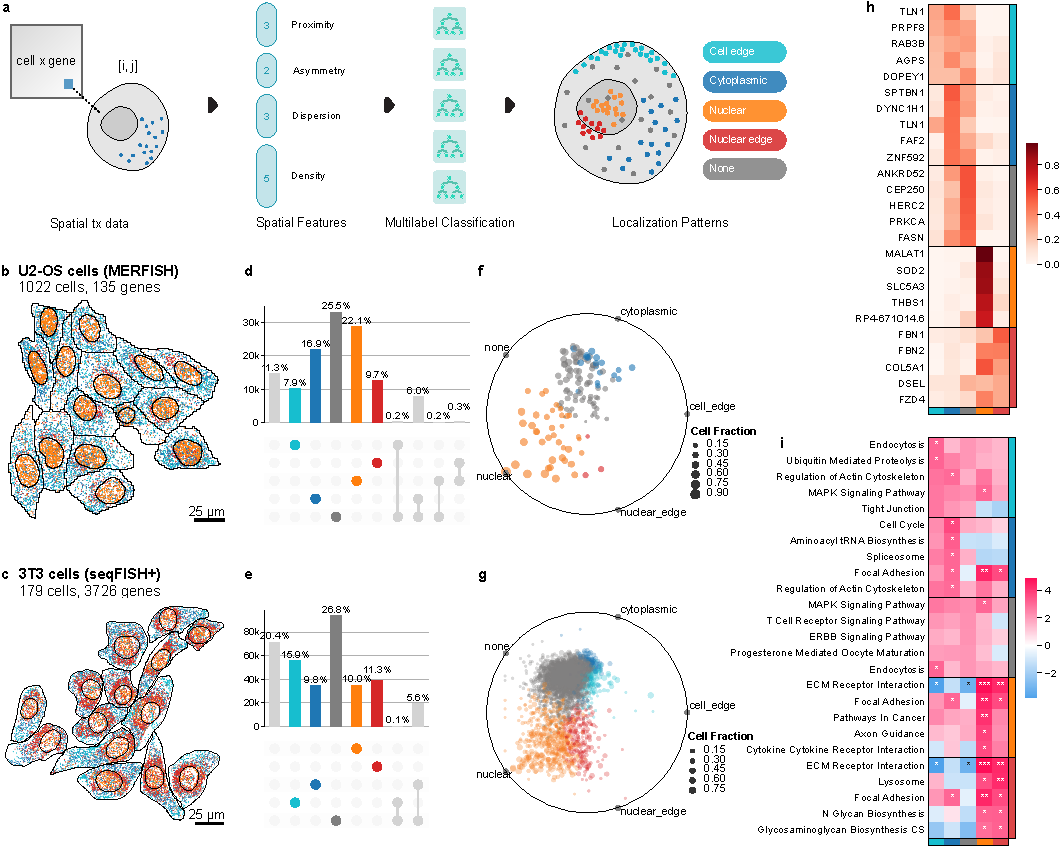
\includegraphics[width=\textwidth]{2_figures-and-files/Fig2.pdf}
    \caption[Subcellular RNA localization changes upon Doxorubicin treatment in iPSC-derived cardiomyocytes]{\textbf{Subcellular RNA localization changes upon Doxorubicin treatment in iPSC-derived cardiomyocytes} A. Cardiomyocytes derived from human iPSCs were treated with DMSO or 2.5 uM DOX for 12 hours. The localizations of 100 genes relevant to cardiomyocyte health and function were measured using Molecular Cartography. Cell boundaries were determined using ClusterMap and nuclei were segmented using Cellpose. B. Top 10 upregulated and downregulated genes in vehicle versus treatment. C. APEX-seq location-specific gene enrichment of fluxmap domains for the cytosol, endoplasmic reticulum membrane (ERM), endoplasmic reticulum lumen (ER Lumen), nuclear lamina, nucleus, nucleolus, nuclear pore and outer mitochondrial matrix (OMM). D. Fluxmap domains visualized for a representative field of view of cardiomyocytes for vehicle and treatment respectively highlighting cellular nuclei, ERM/OMM, ER Lumen, and cytosol. E. RNAflux fluxmap enrichment of each gene averaged across vehicle and treatment cardiomyocytes captures changes in subcellular RNA localization. Visualization of RBM20 F. and CACNB2 G. confirms the depletion of transcripts from the perinuclear and cytosolic compartments of cardiomyocytes upon DOX treatment.}
    \label{fig:Doxorubicin treatment cardiomyocytes}
\end{figure}

\section{Discussion}

In this study of DOX-induced stress in cardiomyocytes, we utilized single-molecule spatial transcriptomics to identify changes in both gene expression and subcellular RNA localization resulting from DOX treatment. Of particular interest was the RNA binding protein RBM20, whose extranuclear depletion in mRNA represents a potential target for therapeutic intervention. This localization behavior may be an early consequence leading to the functional mis-splicing of RBM20's cardiomyopathy-associated targets. Sequestration of the mRNA may be an indirect mechanism of down-regulation. The ERM-associated fluxmap seems to be relatively larger in DOX treated cells compared to vehicle, suggesting that remodeling of organelles may drive movement of molecules or vice versa. 

We found that the 2D spatial resolution of molecular coordinates and segmentation data to limit the clarity of our analyses. While the Clustermap based cell segmentation was sufficient to approximate subcellular domains with RNAflux in the vehicle and 12 hour treatment samples, many regions of the 24 hour and 48 hour treatment samples have denser cells that sit on top of one another due to tighter cell seeding densities. As a result, molecular coordinates and segmentations were flattened to two dimensions, making it impossible to disambiguate expression patterns from overlapping cells. We foresee that better resolution and 3D compatible segmentation algorithms will alleviate this in the future. This is likely required for analysis to achieve subcellular resolution in more complex systems e.g. tissue slices and organoids.

Due to the targeted nature of the particular spatial transcriptomics platform, the 100 gene panel is biased for genes annotated for cardiac function, limiting discovery of novel targets. Expanding the panel size would allow us to capture a better picture of spatial perturbations to the transcriptomic landscape. Additionally, generalizing spatial analyses in Bento from 2D to 3D would enable finer segmentation of subcellular compartments and cells, in turn improving RNA localization analysis. Overcoming these challenges will be useful not only for enabling spatial analysis to other cell lines and conditions, but also to even more heterogeneous systems such as tissue.

\section{Methods}

\subsection{Preprocessing cardiomyocytes datasets}
Single-cell expression matrices of both vehicle replicates and both DOX treatment samples were concatenated as a single expression matrix. Cells were projected into two dimensions with UMAP dimensional reduction. No significant batch effects were detected. Leiden clustering was performed at resolution=0.5 to isolate and filter out a non-myocyte population depleted in SLC8A1 expression (Supp. Fig. 1A). All described preprocessing steps were performed in Scanpy\cite{wolfSCANPYLargescaleSinglecell2018}.

\subsection{RNAflux: Unsupervised spatial embedding and subcellular domain quantization}

For the iPSC-derived cardiomyocytes, a step size of 5 data units was used to compute RNAflux embeddings. Visualization and enrichment of locale-specific transcriptomes derived by APEX-seq were performed as described in Chapter \ref{chap:chapter 1}.

\subsection{Molecular Cartography}
\textit{Cultured cell processing.} After Doxorubicin treatment, cardiomyocytes were washed with PBS (1x) twice and fixed in Methanol (-20°C) for 10 min. After fixation, Methanol was aspirated and cells were dried and stored at -80°C until use. The samples were used for Molecular CartographyTM (100-plex combinatorial single molecule fluorescence in-situ hybridization) according to the manufacturer’s instructions Day 1: Molecular Preparation Protocol for cells,  starting with the addition of buffer DST1  followed by cell priming and hybridization. Briefly, cells were primed for 30 minutes at 37°C followed by overnight hybridization of all probes specific for the target genes (see below for probe design details and target list). Samples were washed the next day to remove excess probes and fluorescently tagged in a two-step color development process. Regions of interest were imaged as described below and fluorescent signals removed during decolorization. Color development, imaging and decolorization were repeated for multiple cycles to build a unique combinatorial code for every target gene that was derived from raw images as described below.
Probe Design. The probes for 100 genes were designed using Resolve's proprietary design algorithm. Briefly, the probe-design was performed at the gene-level. For every targeted gene, all full-length protein coding transcript sequences from the ENSEMBL database were used as design targets if the isoform had the GENCODE annotation tag `basic'\cite{frankishGENCODEReferenceAnnotation2019,yatesEnsembl20202019}. To speed up the process, the calculation of computationally expensive parts, especially the off-target searches, the selection of probe sequences was not performed randomly, but limited to sequences with high success rates. To filter highly repetitive regions, the abundance of k-mers was obtained from the background transcriptome using Jellyfish\cite{marcaisFastLockfreeApproach2011}. Every target sequence was scanned once for all k-mers, and those regions with rare k-mers were preferred as seeds for full probe design. A probe candidate was generated by extending a seed sequence until a certain target stability was reached. A set of simple rules was applied to discard sequences that were found experimentally to cause problems. After these fast screens, the remaining probe candidates were mapped to the background transcriptome using ThermonucleotideBLAST\cite{gansImprovedAssaydependentSearching2008} and probes with stable off-target hits were discarded. Specific probes were then scored based on the number of on-target matches (isoforms), which were weighted by their associated APPRIS level\cite{rodriguezAPPRIS2017Principal2018}, favoring principal isoforms over others. A bonus was added if the binding-site was inside the protein-coding region. From the pool of accepted probes, the final set was composed by picking the highest scoring probes. Probes with catalog numbers can be found in Supp. Table 1\cite{mahBentoToolkitSubcellular2022}. 

\textit{Imaging.} Samples were imaged on a Zeiss Celldiscoverer 7, using the 50x Plan Apochromat water immersion objective with an NA of 1.2 and the 0.5x magnification changer, resulting in a 25x final magnification. Standard CD7 LED excitation light source, filters, and dichroic mirrors were used together with customized emission filters optimized for detecting specific signals. Excitation time per image was 1000 ms for each channel (DAPI was 20 ms). A z-stack was taken at each region with a distance per z-slice according to the Nyquist-Shannon sampling theorem. The custom CD7 CMOS camera (Zeiss Axiocam Mono 712, 3.45 um pixel size) was used. For each region, a z-stack per fluorescent color (two colors) was imaged per imaging round. A total of 8 imaging rounds were done for each position, resulting in 16 z-stacks per region. The completely automated imaging process per round was realized by a custom python script using the scripting API of the Zeiss ZEN software (Open application development).

\textit{Image Processing and Spot Segmentation.} As a first step all images were corrected for background fluorescence. A target value for the allowed number of maxima was determined based upon the area of the slice in um² multiplied by the factor 0.5. This factor was empirically optimized. The brightest maxima per plane were determined, based upon an empirically optimized threshold. The number and location of the respective maxima was stored. This procedure was done for every image slice independently. Maxima that did not have a neighboring maximum in an adjacent slice (called z-group) were excluded. The resulting maxima list was further filtered in an iterative loop by adjusting the allowed thresholds for (Babs-Bback) and (Bperi-Bback) to reach a feature target value (Babs: absolute brightness, Bback: local background, Bperi: background of periphery within 1 pixel). This feature target values were based upon the volume of the 3D-image. Only maxima still in a zgroup of at least 2 after filtering were passing the filter step. Each z-group was counted as one hit. The members of the z-groups with the highest absolute brightness were used as features and written to a file. They resemble a 3D-point cloud. To align the raw data images from different imaging rounds, images had to be registered. To do so the extracted feature point clouds were used to find the transformation matrices. For this purpose, an iterative closest point cloud algorithm was used to minimize the error between two point-clouds. The point clouds of each round were aligned to the point cloud of round one (reference point cloud). The corresponding point clouds were stored for downstream processes. Based upon the transformation matrices the corresponding images were processed by a rigid transformation using trilinear interpolation. The aligned images were used to create a profile for each pixel consisting of 16 values (16 images from two color channels in 8 imaging rounds). The pixel profiles were filtered for variance from zero normalized by total brightness of all pixels in the profile. Matched pixel profiles with the highest score were assigned as an ID to the pixel. Pixels with neighbors having the same ID were grouped. The pixel groups were filtered by group size, number of direct adjacent pixels in group, number of dimensions with size of two pixels. The local 3D-maxima of the groups were determined as potential final transcript locations. Maxima were filtered by the number of maxima in the raw data images where a maximum was expected. Remaining maxima were further evaluated by the fit to the corresponding code. The remaining maxima were written to the results file and considered to resemble transcripts of the corresponding gene. The ratio of signals matching to codes used in the experiment and signals matching to codes not used in the experiment were used as estimation for specificity (false positives). The algorithms for spot segmentation were written in Java and are based on the ImageJ library functionalities. Only the iterative closest point algorithm is written in C++ based on the libpointmatcher library (https://github.com/ethz-asl/libpointmatcher).

\textit{Image segmentation.} Cellpose v1.0.2\cite{stringerCellposeGeneralistAlgorithm2021} was used to perform image segmentation to determine the boundaries of nuclei. The nuclei boundaries were determined by running Cellpose with the `nuclei' model using default parameters on the DAPI stain channel of the pre-hybridization images. Cytoplasm boundaries were determined with ClusterMap\cite{heClusterMapMultiscaleClustering2021} using spot coordinates.

\subsection{iPSC Cardiac Differentiation and Doxorubicin Treatment}
Matrigel (Corning, cat \# 354277) coated plates were used to culture iPSCs with mTESR Plus human iPSC medium (StemCell Technologies, cat \# 100-0276) in a humidified incubator at 37°C with 5\% CO2. iPSCs were dissociated with Gentle Cell Dissociation Reagent (StemCell Technologies, cat \# 100-0485) and passaged with mTESR Plus medium and 10uM ROCK inhibitor (Tocris, cat \#1254) at a ratio of 1:12. mTESR plus medium was replaced every other day until the cells reached 80\% confluency for maintenance and replating, or 90\% confluency for cardiac differentiation utilizing a chemically defined protocol\cite{lianRobustCardiomyocyteDifferentiation2012}. On day 0 of cardiac differentiation, cells were treated with 6uM CHIR99021 (Selleck Chem, cat \# S1263) in RPMI 1640 media (Gibco, cat \# 11875) and B27 minus insulin supplement (Thermo Fisher, cat \# A1895601). On day 2, CHIR was removed, and cells were cultured with RPMI 1640 media and B27 minus insulin supplement (Thermo Fisher, cat \# A18956). On day 3, media was replaced with RPMI media containing B27 minus insulin supplement and 5 uM Wnt-C59 (Cellagen Technologies, cat \# C7641-2s). On days 5, 7, and 9, media was replaced with RPMI media containing B27 insulin supplement (Thermo Fisher, cat \# 17504). On days 11 and 13, media was replaced with RPMI 1640 media without glucose (Thermo Fisher, cat \# 11879020) containing B27 insulin supplement for purification of cardiomyocytes. From days 15 onward, the cells were cultured in RPMI 1640 media containing B27 supplement which was changed every other day until the cells reached day 30 for replating. For replating, cells were incubated in 10X TrypLE (Thermo Fisher, cat \# A1217701) for 12 minutes at 37 C, neutralized with equal volumes of RPMI 1640 media containing B27 supplement with 20\% FBS (Gibco, cat \# 26140-079), gently dissociated by pipetting, then spun down and resuspended for replating in RPMI 1640 media containing B27 supplement with 20\% FBS. The next day, the cell media was replaced with RPMI 1640 media containing B27 supplement which was replaced with fresh media every other day. On day 48 the cells were replated onto chamber slides (Ibidi, cat \# 80826) as described above and recovered for 10 days before doxorubicin treatments began (MedChemExpress, cat \# HY-15142). On day 60, doxorubicin treatments concluded, and the cells underwent methanol fixation.

\subsection{Data Availability}
Preprocessed data for Molecular Cartography profiled cardiomyocytes is deposited at https://doi.org/10.6084/m9.figshare.c.6564043.v1 and is accessible through the Bento Python package. 

\subsection{Code Availability}
Analysis code for generating figures can be found at: https://github.com/ckmah/bento-manuscript.

\subsection{Acknowledgements}

As this work was derived from the same manuscript, see \ref{chap:chapter 1} for corresponding details.

\subsection{Author Contributions}
As this work was derived from the same manuscript, see \ref{chap:chapter 1} for corresponding details.

\subsection{Competing Interests}
As this work was derived from the same manuscript, see \ref{chap:chapter 1} for corresponding details.